\section{Matrix Multiplication using Pthread}

\begin{itemize}

    \item {
        \textbf{병렬화 방식.}
        주어진 행렬은 row-wise 방식으로 메모리를 사용한다 (바로 다음 메모리가 같은 row의 다음 element).
        이를 고려할 때 행렬 B를 쪼개는 것이 행렬 A에 대한 캐시 활용도를 높일 수 있을 것이라고 판단하였다.
        이에 각 thread가 행렬 A를 모두 사용하고 행렬 B의 일부 column을 사용하여 행렬 C의 일부 column을
        계산하도록 코드를 작성하였다.

        Thread를 사용한 병렬화는 OpenMP를 사용하였다.
        계산 중간에 thread 사이의 synchronization은 일어나지 않으며, 각 thread의 계산이 끝나는
        시점이 균일하도록 각 thread에게 행렬 C의 column을 균등히 할당하였다.
        
        또한, 한 번에 행렬 C의 $64 \times 64$ 만큼을 계산하도록 하는 macro kernel을 정의하여
        연산 과정이 cache-friendly 하도록 하였다. Macro kernel 내부에서는 AVX512 코드를 사용하여
        연산을 가속하였다.
    }
    \item {
        \textbf{OpenMP의 Thread 생성.}
        유저는 OpenMP 구문을 사용하여 각 thread가 수행할 일, 분배 방식, synchronization,
        데이터 영역의 속성에 대한 정보를 제공한다. 그러면 컴파일러는 주어진 조건들을 바탕으로
        실제 multithreaded 방식으로 동작하는 코드를 생성한다.
        이 코드에는 각 thread가 수행할 일과 그때 필요한 데이터 영역이 유저가 지정한 대로 구현되어 있으며,
        이에 더해 각 thread를 생성하고, 멈추고, 깨우고, 끝내거나 동기화하는 등의 관리 코드도 포함되어 있다.
        이러한 코드 중 많은 부분이 런타임 라이브러리의 함수를 호출하는 방식으로 구현된다.
        런타임 라이브러리에는 이러한 OpenMP의 user-level 또는 run-time routine에 대한 실제 구현이 들어있다.

        예를 들어 다음과 같은 코드를 컴파일한다고 하자.

        \begin{verbatim}
    #pragma omp parallel for reduction (+:sum) private (x)
    for (i = 1; i <= num_steps; i++)
    { 
        …
        sum = sum + x;
    }
        \end{verbatim}

        이를 컴파일하면 다음과 같은 코드로 변환된다.
        \begin{Verbatim}[commandchars=\\\{\}]
    float \textcolor{blue}{local_sum};
    …
    \textcolor{blue}{ompc_static_init (tid, lower, uppder, incr,.);}
    for (i = lower; i < upper; i += incr)
    \{ 
        …
        local_sum = local_sum + x;
    \}
    \textcolor{blue}{ompc_barrier();}
    \textcolor{blue}{ompc_critical();}
    \textcolor{blue}{sum = (sum + local_sum);}
    \textcolor{blue}{ompc_end_critical();}
        \end{Verbatim}
        
        이때 각종 OpenMP run-time routine을 호출함으로써 주어진 코드를 병렬화하고 동기화하는 모습을
        확인할 수 있다\cite{chapman2015openmp}.
    }
    \item {
        \begin{figure}[t]
            \centering
            \begin{subfigure}[b]{0.49\textwidth}
                \centering
                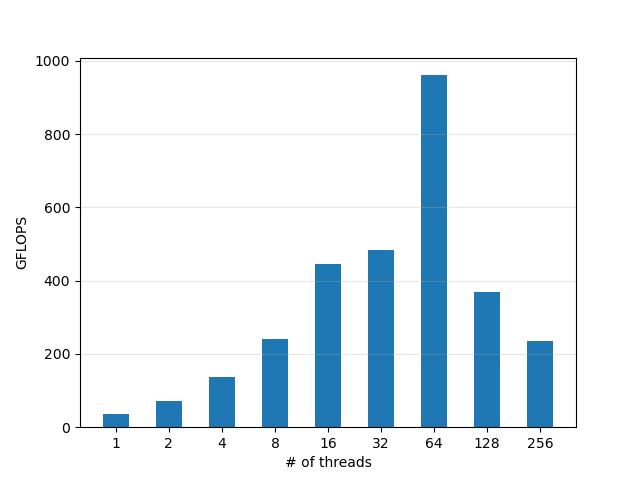
\includegraphics[width=\textwidth]{imgs/gflops_exp.png}
                \caption{Thread를 2배씩 늘린 경우.}\label{fig:gflops_exp}
            \end{subfigure}
            \hfill
            \begin{subfigure}[b]{0.49\textwidth}
                \centering
                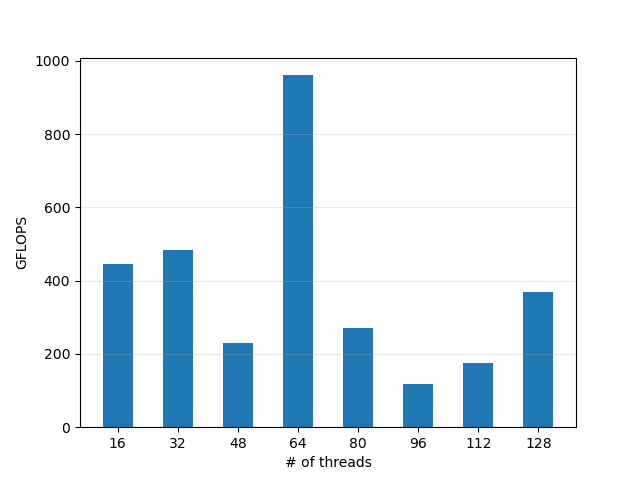
\includegraphics[width=\textwidth]{imgs/gflops_lin.png}
                \caption{Thread를 16개씩 늘린 경우.}\label{fig:gflops_lin}
            \end{subfigure}
            \caption{Thread 수에 따른 성능 변화.}\label{fig:gflops}
        \end{figure}
        
        \textbf{Thread 수와 행렬곱 성능.}
        Thread를 2배씩 증가시키며 실험한 결과[Fig.~{\ref{fig:gflops_exp}}],
        GFLOPS는 증가하다가 다시 감소하는 모습을 보였다.
        처음에 증가하는 이유는 아직 physical core의 수보다 thread의 수가 적기 때문에 thread가 증가함에 따라
        새로운 physical core가 연산에 참여할 수 있게 되기 때문이다.
        64개 thread를 넘어서면 다시 감소하는 모습을 보이는데, 이때부터는 logical core의 수보다
        thread의 수가 많아지면서 여러 thread가 한 core를 두고 경쟁하게 되기 때문이며,
        그 과정에서 overhead가 발생하여 성능이 감소하게 된다.

        추가로, 최고 성능을 보인 thread 수의 근처에서 thread의 수를 16씩 증가시키며 실험해본 결과
        [Fig.~{\ref{fig:gflops_lin}}], 훨씬 일관되지 않은 모습을 보였다.
        이는 thread의 수가 logical core의 수의 약수 또는 배수가 아닌 경우 경쟁이 매우 복잡하게 일어난다는 점과,
        thread의 수에 비례하여 경쟁 자체가 더 치열해지는 두 가지 요인이 동시에 작용한 결과이다.
    }
    \item {
        \textbf{최적의 Thread 수.}
        위 실험에서 확인한 바, 64개의 thread를 사용할 때 압도적인 최고 성능을 보였으며
        이 때의 성능은 961.032611 GFLOPS이다.
        이는 이론적으로 계산한 peak performance인 2150.4 GLOPS의 44.7\%에 해당한다.

        최고 성능을 보인 thread의 수는 CPU의 logical core의 수와 같다. 그 이유로 추측되는 것은,
        matrix multiplication을 위해서는 실제 연산을 수행하는 명령어 뿐 아니라
        메모리에 접근하는 명령어와 같은 여러 가지 명령어들 또한 자주 수행되기 때문이다.
        따라서 두 개의 thread에서 수행되는 연산들이 interleave될 여지가 많았을 것으로 보이며,
        그에 따라 logical core의 수인 64개의 thread를 사용한 경우에 가장 좋은 성능을 보인 것으로 보인다.
        만약 실제 연산을 수행하는 명령어 이외의 명령어들의 비율이 매우 적어진다면, 
        physical core의 수인 32개의 thread를 사용하는 것이 가장 좋은 성능을 보이게 될 것이다.

        \textbf{개선 방법.}
        더 높은 성능을 위해 적용할 수 있는 방법은 다음과 같은 것들이 있다.
        이 중 몇몇은 제출한 코드를 컴파일할 때 자동으로 적용될 수 있는 것이지만,
        최적화된 성능을 얻기 위해서는 어셈블리 코드 수준에서 일일이 적용해주어야 한다.
        
        \begin{itemize}
            \item {
                연산을 수행하는 최하단 커널에 loop-unroll을 적용한다. 이를 통해 루프를 수행하기 위해
                기본적으로 존재하는 overhead를 효과적으로 줄일 수 있으며, 컴파일러에게 더 많은
                최적화 기회를 제공할 수 있다.
            }
            \item {
                Macro kernel과 micro kernel을 분리한다. 보통의 GEMM 라이브러리에서는 cache의 사용과
                register의 사용을 최적화하기 위해 여러 단계의 kernel을 정의하여 사용한다.
                이번 과제에서는 적당한 크기의 macro kernel과 매우 naive한 micro kernel을
                사용하였으나, 프로세서의 캐시를 고려하여 macro kernel의 크기를 설정하고,
                매우 최적화된 micro kernel을 사용한다면 성능을 매우 높일 수 있다.
            }
            \item {
                연산 이전에, 주어진 행렬을 연산에 최적화된 배열로 buffer에 복사한다.
                이를 통해 micro kernel에서 연산을 더욱 효과적으로 수행할 수 있으며,
                연산 이전에 데이터에 접근하게 되므로 연산 수행 시에 cache의 hit-rate가 증가한다.
            }
            \item {
                프로세서가 superscalar 방식으로 동작하는 경우, micro kernel에서 memory load 및
                prefetch 명령어와 실제 연산 명령어를 적절한 비율로 섞어주는 기법을 사용할 수 있다.
                연산을 수행하는 과정에서도 사용이 끝난 레지스터를 다음에 사용할 값으로 미리 채워주거나,
                곧 사용하게 될 데이터를 prefetch 하여 캐시에 유지하도록 하는 등의 명령어를 수행해야 한다.
                이러한 명령을 실제 연산 명령어 사이에 일정 주기로 삽입하여 memory access latency를
                효과적으로 숨길 수 있다.
            }
        \end{itemize}
    }
    \item {
        \begin{figure}[t]
            \centering
            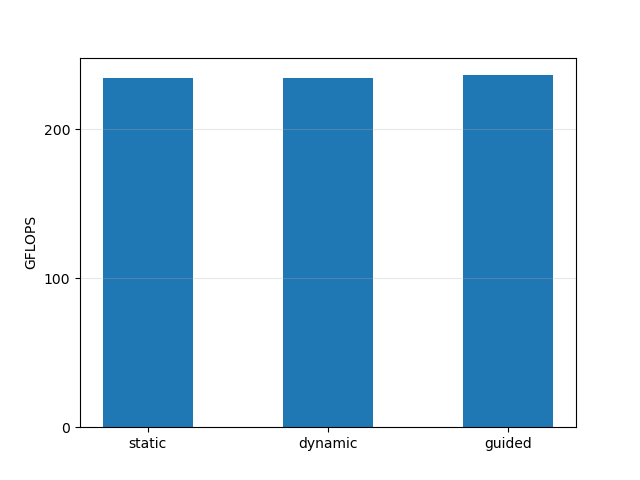
\includegraphics[width=0.6\textwidth]{imgs/schedule_policy.png}
            \caption{Schedule 방식에 따른 FLOPS 차이.}\label{fig:schedule_policy}
        \end{figure}

        \textbf{OpenMP의 Loop Scheduling.}
        OpenMP에서는 for loop의 scheduling 방식을 \texttt{static}, \texttt{dynamic}, \texttt{guided}
        중 선택할 수 있다.
        \texttt{static}의 경우, 전체 루프 카운트를 각 thread에 균등하게 분배한다.
        예를 들어 100번의 루프를 4개의 thread로 수행한다면, 각 thread는 25번의 루프를 수행하게 된다.
        \texttt{dynamic}의 경우, 작업을 수행할 준비가 된 thread에게 그때그때 루프를 할당한다.
        \texttt{guided}의 경우, \texttt{dynamic}과 비슷하게 각 thread에게 루프를 동적으로 할당하지만,
        시간이 지날수록 배분하는 양이 점차 줄어든다는 차이가 있다.
        이를 통해 처음에는 분배로 인한 overhead를 줄일 수 있고,
        작업이 끝날 즈음에는 thread 사이의 workload가 불균등해지는 것을 방지할 수 있다.

        행렬곱을 분배하는 for loop의 크기를 네 배로 늘리고 각 loop에서 수행하는 연산의 크기를 1/4로 줄인 후,
        세 가지 방식을 사용하여 \texttt{run\_performance.sh} 스크립트로 실험한 결과[Fig.~\ref{fig:schedule_policy}],
        유의미한 차이를 찾을 수 없었다. 그 이유는 각 loop의 연산의 크기가 매우 균일하고 작기 때문에
        각 thread에 분배되는 workload의 크기가 scheduling 방식의 차이로 인해 크게 차이나지 않았기 때문이다.
    }
    
\end{itemize}